\documentclass{article}
\usepackage{enumerate}
\usepackage{amsmath}
\usepackage{amssymb}
\usepackage{graphicx}
\usepackage{subfigure}
\usepackage{geometry}
\usepackage{caption}
\usepackage{indentfirst}
\usepackage{listings}
\usepackage{xcolor}  
\geometry{left=3.0cm,right=3.0cm,top=3.0cm,bottom=4.0cm}
\allowdisplaybreaks[4]
\title{VE216 Lab1}
\author{Liu Yihao 515370910207}
\date{}
\lstset{
	language=Matlab, numbers=left, tabsize=4,
	framexleftmargin=1.5mm, frame=leftline,
	keywordstyle=\color{blue}\bfseries,
	identifierstyle=\bf, breaklines=true, 
	basicstyle=\normalsize,rulecolor=\color{brown}, 
	numberstyle=\color[RGB]{20,20,20}
}
\begin{document}
\vspace*{0.25cm}

\hrulefill

\thispagestyle{empty}

\begin{center}
\begin{large}
\sc{UM--SJTU Joint Institute \vspace{0.3em} \\ Intro to Signals and Systems \\(VE216)}
\end{large}

\hrulefill

\vspace*{5cm}
\begin{Large}
\sc{{Laboratory Report}}
\end{Large}

\vspace{2em}

\begin{large}
\sc{{Lab 1
\vspace{0.5em}

LTI Systems}}
\end{large}
\end{center}

\vfill

\begin{table}[h!]
\flushleft
\begin{tabular}{lll}
Name: Zou XiaoFeng \hspace*{2em}&
ID: 515370910179\hspace*{2em}
& Group: 13\\
Name: Shen Haonan \hspace*{2em}&
ID: 515370910150\hspace*{2em}
& Group: 13\\
Name: Liu Yihao \hspace*{2em}&
ID: 515370910207\hspace*{2em}
& Group: 13\\
\\

Date: 7 April 2017 

\end{tabular}
\end{table}

\hfill

\newpage

\section{Objectives}
\begin{itemize}
	\item To become familiar with the laboratory equipment: power supply, signal generator, digital oscilloscope,
computer data acquisition system (Scope Connect).
	\item To review basic concepts of linear time-invariant systems.
	\item To illustrate several possible ways to determine the impulse response of a physical system from measured
data.
	\item To use linearity, time-invariance and impulse response to compute the output of an LTI system when
the input is a step, a pulse, or a more complicated signal. You will compare these calculations with
actual measurements.
	\item To measure the frequency response of an LTI system and compare against theory.
\end{itemize}

\section{Theoretical background}
An RC circuit is used so that the computations are easy and physically meaningful. The same procedures
can be applied to much more complicated systems.

\subsection{RC circuit}
The RC circuit shown below is an example of a simple LTI system. Of course, there are many other LTI
systems that do not involve circuits at all.

\begin{figure}[htbp]
	\centering
	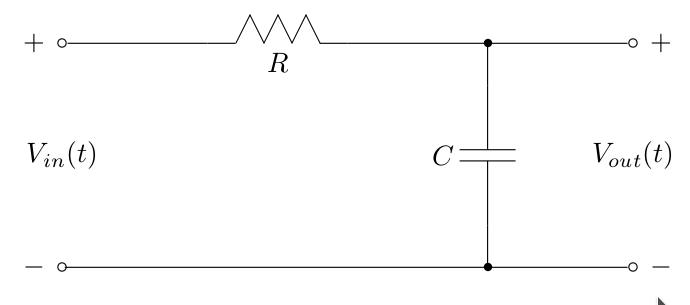
\includegraphics[width=0.7\linewidth]{fig-1.png}
	\caption{RC circuit}
	\label{fig-setup}
\end{figure}

We will take the system input to be the voltage $V_{in}(t)$, while the system output is the voltage, $V_{out}(t)$,
dropped across the capacitor. Notice that these voltages, in general, will be functions of time, $t$.

\subsection{When is a linear circuit a linear system?}

Using Kirchoffs current and voltage laws, one can easily derive a differential equation model of the RC-circuit
in Figure \ref{fig-setup}, namely

\begin{equation}
	RC\frac{dV_{out}(t)}{dt}+V_{out}(t)=V_{in}(t)
\end{equation}

Appealing to basic knowledge of ODEs from a sophomore level math course, the total solution is seen to be

\begin{equation}
	V_{out}(t)=V_0e^{-t/RC}+\int_0^t\frac{1}{RC}e^{-(t-\tau)/RC}V_{in}(\tau)d\tau,\quad t\geqslant0
\end{equation}

where the initial condition at time zero is $V_{out}(0)=V_0$. It is very easy to verify that $V_{out}(t)$ is a linear
function $V_{in}(t)$ if, and only if, $V_{out}(0)=V_0=0$, that is, the initial voltage on the capacitor has to be zero.
This point is emphasized because you will have to assure this in the laboratory by either waiting for the
charge to decay on the capacitor or by shorting the capacitor with a wire.\\

\textbf{Reassuring remark:} We will learn how to deal comfortably with nonzero initial conditions when we
study the Laplace transform. For the time being, it is important to realize that we are assuming zero initial
conditions when our models arise from a differential equation.

\subsection{Impulse Response}

The impulse response, $h(t)$, of an LTI system is, by definition, the output response when the input of the
system is a delta function, $\delta(t)$. Of course, the delta function is a mathematical idealization. In practice,
$h(t)$ can be well approximated by the response of the system when the input is a pulse of very short duration (compared with the response time of the system) and unit area, such as $p_\delta(t)=\dfrac{1}{\delta}(u(t)-u(t-\delta))$ for $\delta>0$ sufficiently small.

Note that in order to keep the area of the pulse equal to unity, the amplitude has to increase as the pulse
duration gets shorter. Often, this is a problem in a practical system as a large voltage pulse may fry an
amplifier, for example. One way to get around this is to use linearity and realize that if the input is scaled
by ``$b$'', then the output will be scaled by ``$b$'' as well. Consequently, if the measured response is divided by
``$b$'', an approximation of the impulse response is obtained.

\subsection{Step Response}
For any LTI system the output can be expressed as

\begin{equation}
	y(t)=x(t)*h(t)=\int_{-\infty}^{+\infty}x(\tau)h(t-\tau)d\tau=\int_{-\infty}^{+\infty}x(t-\tau)h(\tau)d\tau
\end{equation}

where $x(t)$ denotes the input and ∗ denotes the convolution operation. The output resulting when the input
is a unit step function, $x(t) = u(t)$, is called the unit step response. Simple manipulation leads to

\begin{equation}
	y_{step}(t)=u(t)*h(t)=\int_{-\infty}^{+\infty}h(\tau)u(t-\tau)d\tau=\int_{-\infty}^th(t-\tau)u(\tau)d\tau+\int_t^{+\infty}h(t-\tau)u(\tau)d\tau
\end{equation}

which, because the unit step function is equal to $1$ for $t − τ > 0$ and equal to $0$ for $t − τ < 0$ step response
simplifies to

\begin{equation}
	y_{step}(t)=\int_{-\infty}^th(\tau)d\tau
\end{equation}

By taking the derivative of $y_{step}(t)$ with respect to $t$, we obtain, by the fundamental theorem of calculus,

\begin{equation}
	\frac{dy_{step}(t)}{dt}=\frac{d}{dt}\int_{-\infty}^th(\tau)d\tau=h(t)
\end{equation}

Thus the impulse response can be computed from the unit step response by calculating the derivative of the
step response with respect to time. This is a useful observation because it is sometimes easier to apply a
step input to a physical system than it is to apply (an approximation of) an impulse.

We now have two ways of determining the impulse response from data. A third way will be hinted at a
little later.

\section{Experiment procedures}
\subsection*{Setup}
\begin{itemize}
	\item Function generator: Utility $\rightarrow$ Output Setup $\rightarrow$ Load $\rightarrow$ High Z
	\item Oscillator: Trigger Menu 
	$\rightarrow\left\{
	\begin{aligned}
		&\rm 1.Trigger\ Mode \rightarrow Basic \\
		&\rm 2.Edge\ Trigger\ (Rising\ Edge) \\
		&\rm 3.Trigger\ Settings \rightarrow DC\ Coupling
	\end{aligned}
	\right.$
	\item RC circuit: $R = 1 K\Omega$, and $C = 1 \mu F$
\end{itemize}

\subsection{Step Response}
\begin{itemize}
	\item Function generator:\\
	Square wave \qquad Vpp: 1V \qquad frequency: 100Hz
	\item Oscillator:\\
	CH1: 200mV/div \qquad CH2: 200mV/div \qquad Time: 2ms
	\item Bonus: Compare your results with the ideal case
\end{itemize}

\subsection{Pulse Response}
\begin{itemize}
	\item Function generator: Pulse frequency: 100Hz
	\begin{enumerate}
		\item Width: 1ms \qquad A: 100mV
		\item Width: 0.5ms \qquad A: 200mV
	\end{enumerate}
\end{itemize}

\subsection{Ramp Response}
\begin{itemize}
	\item Function generator:\\
	Ramp \qquad Vpp: 100mV \qquad frequency: 100Hz
\end{itemize}

\subsection{Sine Response}
\begin{itemize}
	\item Function generator: 10 Vpp
	\begin{center}
		\begin{tabular}{|c|c|c|c|}
			\hline
			Frequency (Hz) & Vout / Vin & Time Shift & Phase Shift \\
			\hline
			50 &&&\\
			\hline
			500 &&&\\
			\hline
			5k &&&\\
			\hline
		\end{tabular}
	\end{center}
	\item Bonus: Compare your results with ideal case
\end{itemize}

\section{Experimental results}

\subsection{Step Response}
The figure was shown in Figure \ref{fig-1}.

\begin{figure}[htbp]
	\centering
	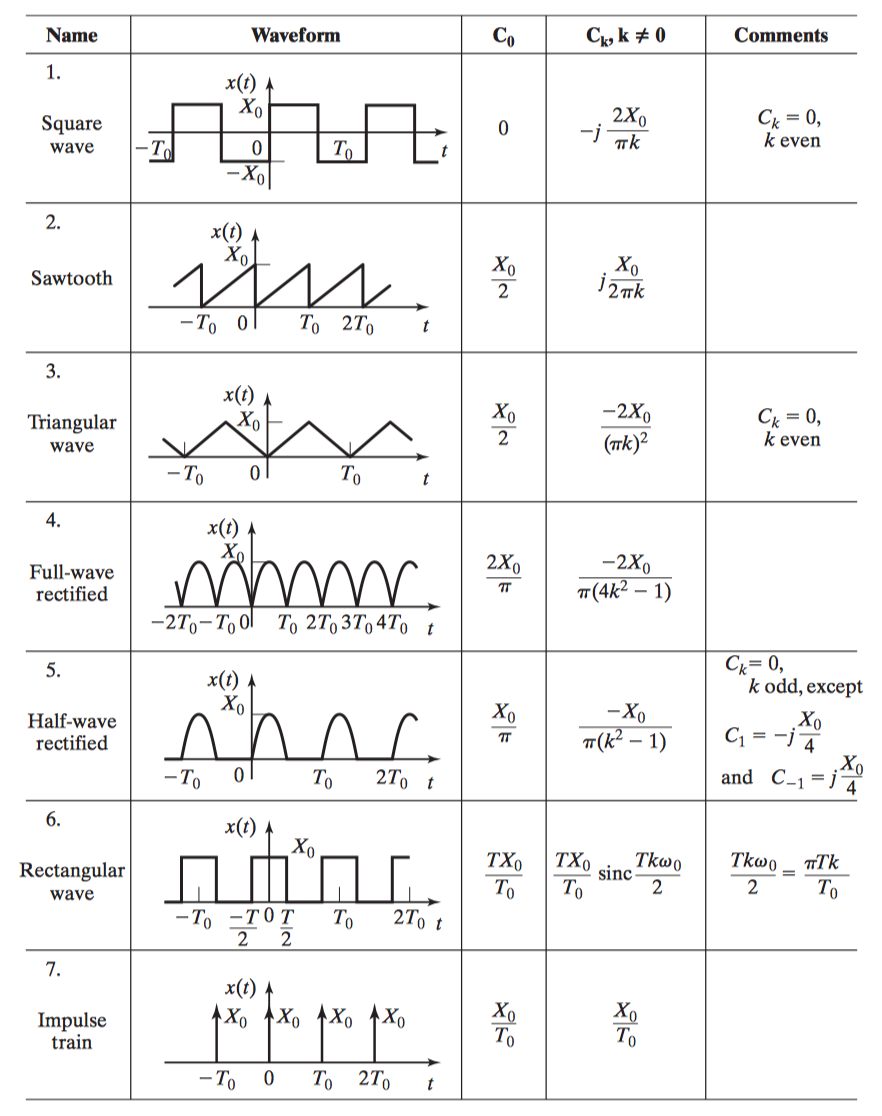
\includegraphics[width=0.7\linewidth]{1.bmp}
	\caption{Step Response}
	\label{fig-1}
\end{figure}

\subsection{Pulse Response}
The figure was shown in Figure \ref{fig-2}.

\begin{figure}[htbp]
	\centering
	\subfigure[Width: 1ms, A: 100mV]{
		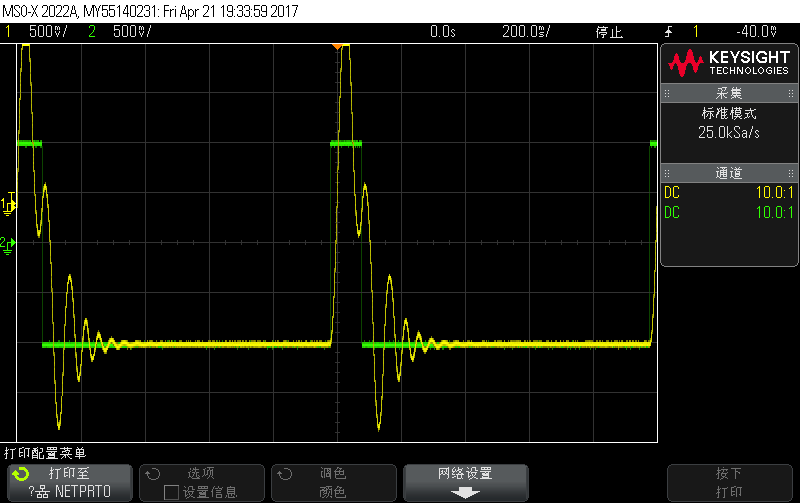
\includegraphics[width=0.45\linewidth]{2.1.bmp}
		\label{fig-2-1}
	}
	\subfigure[Width: 0.5ms, A: 200mV]{
		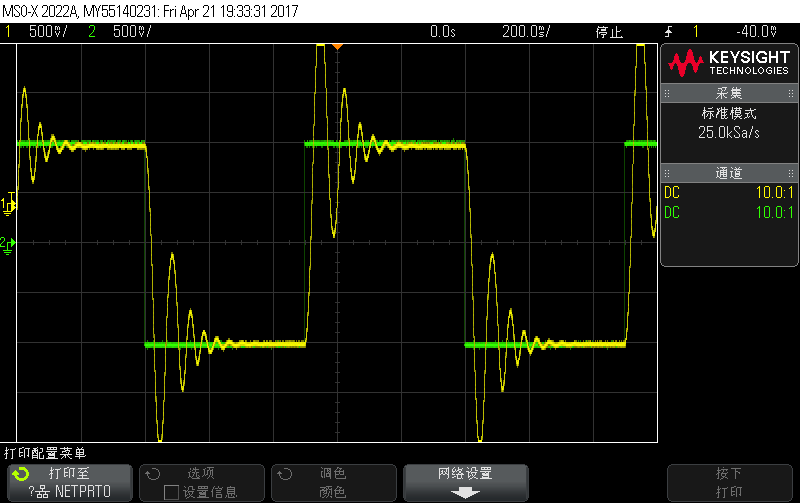
\includegraphics[width=0.45\linewidth]{2.2.bmp}
		\label{fig-2-2}
	}
	\caption{Pulse Response}
	\label{fig-2}
\end{figure}

\subsection{Ramp Response}
The data was shown in Table \ref{fig-3}.

\begin{figure}[htbp]
	\centering
	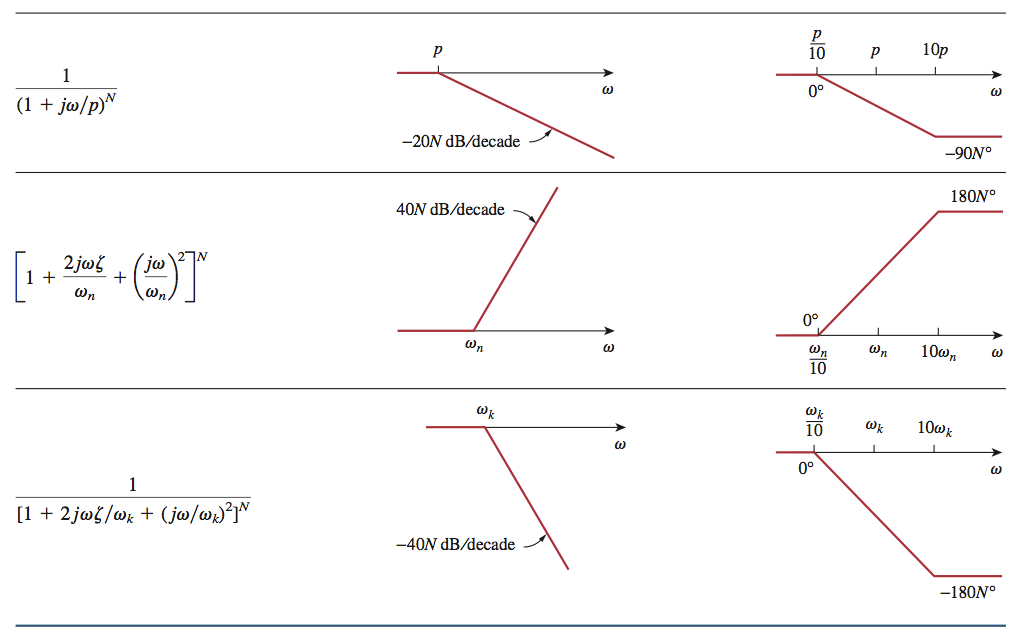
\includegraphics[width=0.7\linewidth]{3.bmp}
	\caption{Ramp Response}
	\label{fig-3}
\end{figure}

\subsection{Sine Response}
The data was shown in Table \ref{tab-4}.

\begin{table}[htbp]
	\centering
	\begin{tabular}{|c|c|c|c|}
		\hline
		Frequency (Hz) & Vout / Vin & Time Shift ($\mu s$) & Phase Shift ($^\circ$) \\
		\hline
		50 & 10.2 / 10.6 = 0.9623 & 880 & -15.84 \\
		\hline
		500 & 3.12 / 10.2  = 0.3059 & 380 & -68.40 \\
		\hline
		5k & 0.385 / 10.1 = 0.0381 & 46 & -82.80\\
		\hline
	\end{tabular}
	\caption{Sine Response}
	\label{tab-4}
\end{table}

In this table, phase shift is calculated according the equation

$$\sphericalangle=-2\pi f_c\Delta t RC \frac{180}{\pi}=-f_c\Delta t\cdot 3.6\times10^{-4}$$

\newpage

\section{Error analysis and discussion}
\subsection{Step Response}
In ideal situation, we know
$$V_{in}(t)=u(t)$$
$$V_{out}(t)=y_{step}(t)=(1-e^{-t/RC})u(t)$$

Then we can substitute $R=1k\Omega$, $C=1\mu F$ into $y_{step}(t)$ and plot the ideal graph when $t\in[0,0.005)$ in MATLAB, as Figure \ref{fig-1-ideal}.

\begin{figure}[htbp]
	\centering
	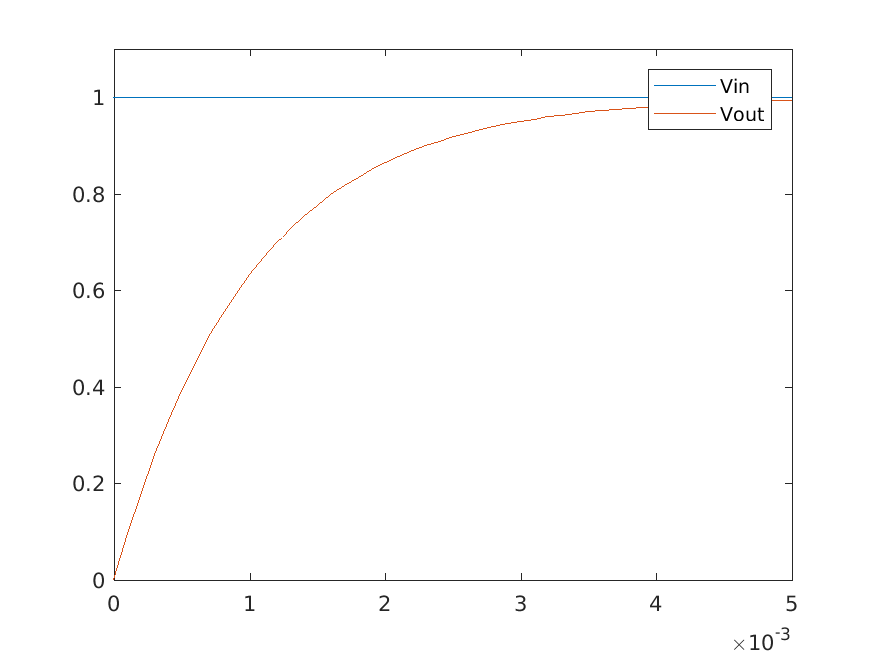
\includegraphics[width=0.7\linewidth]{ideal_1.png}
	\caption{Ideal graph of step response}
	\label{fig-1-ideal}
\end{figure}

We can find that in Figure \ref{fig-1} (experimental), $V_{in}(t)$ was not a straight line, it is probably because of the inner resistance of the experiment instruments. The shape of $V_{out}(t)$ in two figures are very similar.

\subsection{Pulse Response}
In the experiment, we can only simulate a $\delta$ function since instantaneous time period doesn't exist in real world. However, the smaller time period (width) we get, the more accurate the experiment is. \\

The ideal graphs of $h(t)$ with a width were shown in Figure \ref{fig-2-ideal-width}. They are similar to those in the experiment.\\


\begin{figure}[htbp]
	\centering
	\subfigure[Width: 1ms, A: 100mV]{
		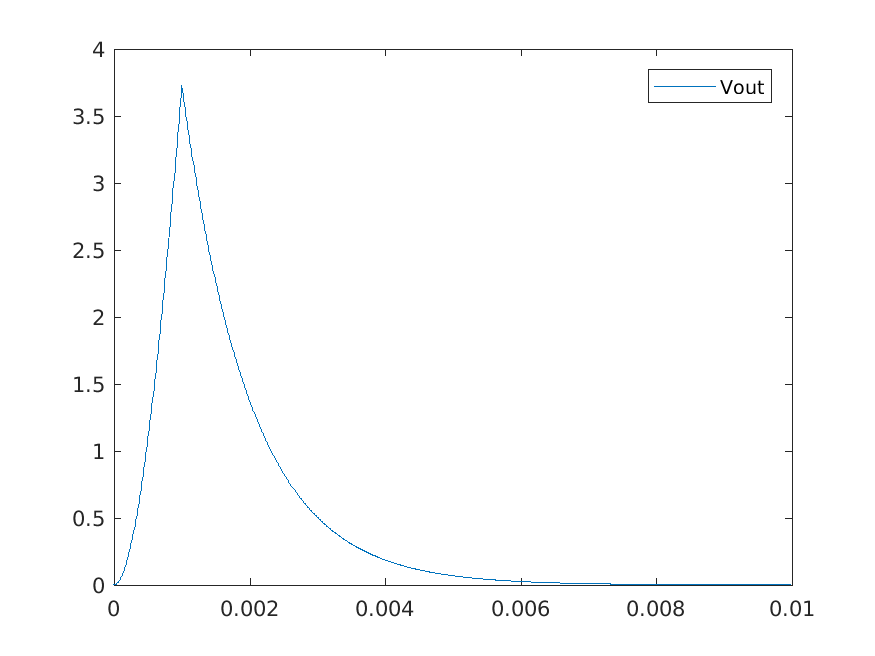
\includegraphics[width=0.45\linewidth]{ideal_2_width_1.png}
		\label{fig-2-ideal-width-1}
	}
	\subfigure[Width: 0.5ms, A: 200mV]{
		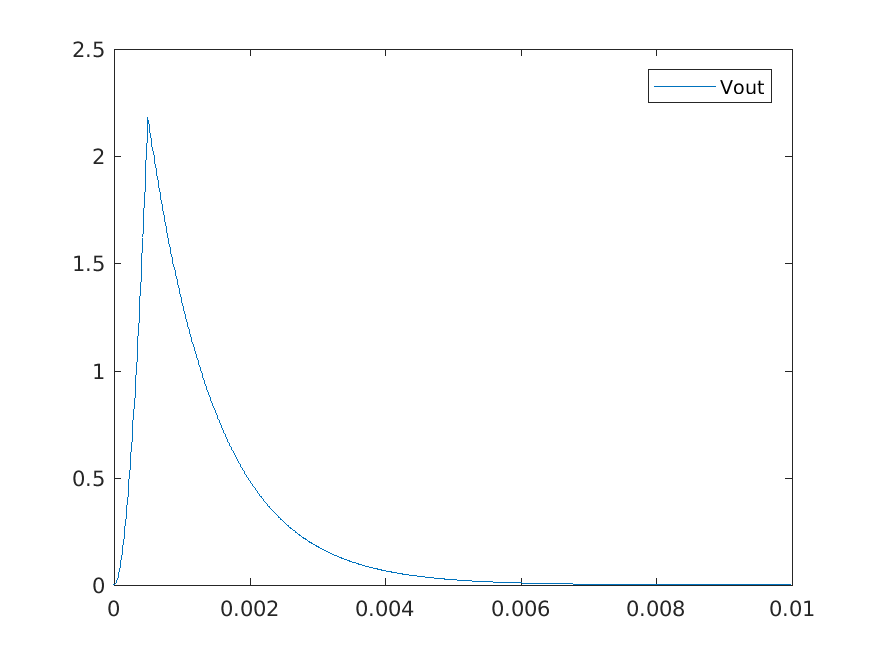
\includegraphics[width=0.45\linewidth]{ideal_2_width_2.png}
		\label{fig-2-ideal-width-2}
	}
	\caption{Ideal Pulse Response in experiment}
	\label{fig-2-ideal-width}
\end{figure}

We know the equation of the pulse response is

$$h(t)=\frac{dy_{step}(t)}{dt}=\frac{1}{RC}e^{-t/RC}u(t)$$

The ideal graph of $h(t)$ was shown in Figure \ref{fig-2-ideal}. It is similar to the figure when width $\to 0$.

\begin{figure}[htbp]
	\centering
	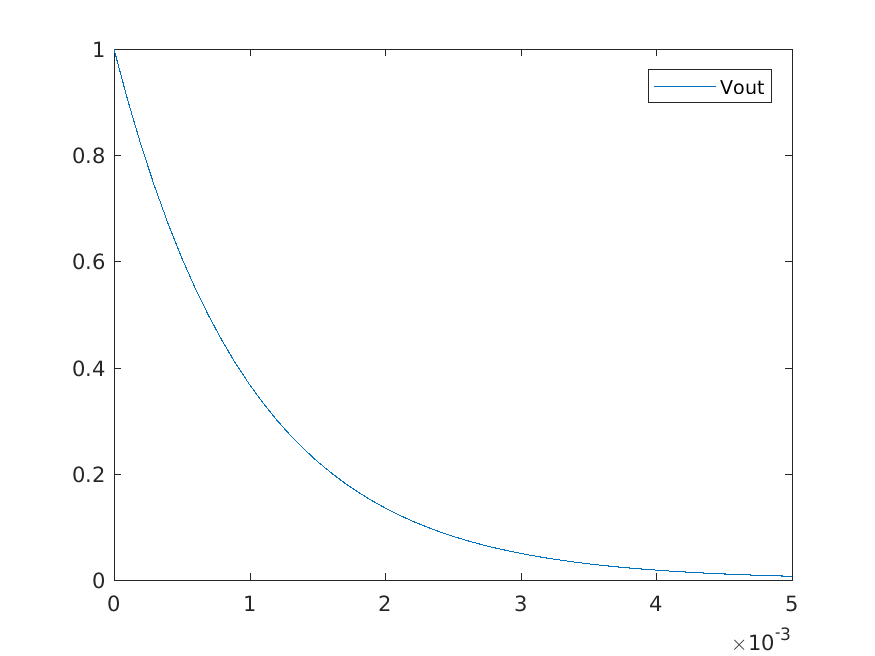
\includegraphics[width=0.7\linewidth]{ideal_2.png}
	\caption{Ideal graph of pulse response}
	\label{fig-2-ideal}
\end{figure}

\newpage

\subsection{Ramp Response}

A period of the ramp function in this experiment is
$$x(t)=\frac{0.1}{0.01}(t-0.005)=10(t-0.005)$$
$$y(t)=x(t)*h(t)$$
The ideal graph of $y(t)$ was shown in Figure \ref{fig-3-ideal}. It fits the figure in the experiment well.

\begin{figure}[htbp]
	\centering
	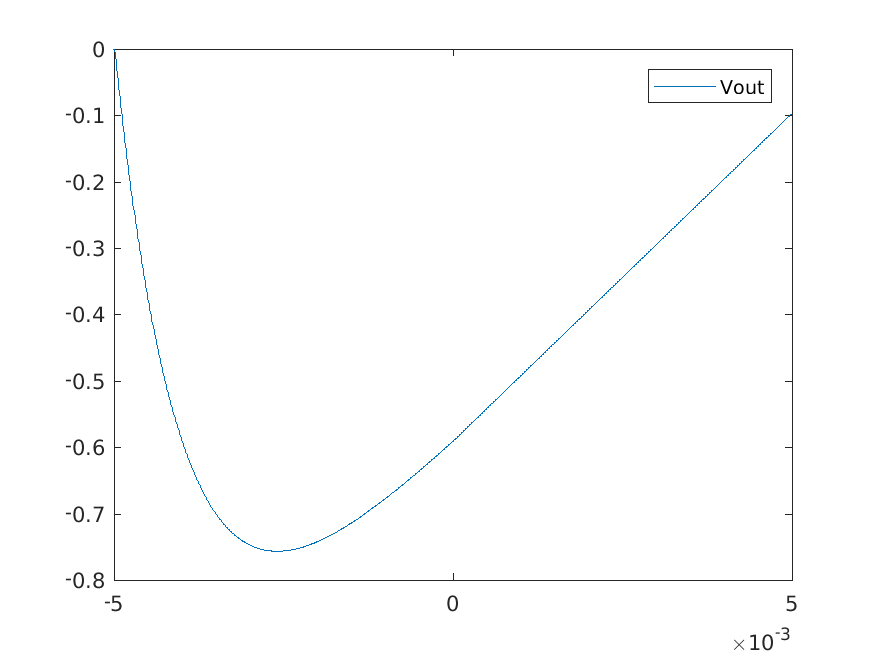
\includegraphics[width=0.7\linewidth]{ideal_3.png}
	\caption{Ideal graph of ramp response}
	\label{fig-3-ideal}
\end{figure}

\subsection{Sine Response}

Theoretically, we have
$$\frac{V_{out}}{V_{in}}=\sqrt{1+(2\pi f_cRC)^2}$$
$$\Delta t=\frac{\arctan(2\pi f_cRC)}{2\pi f_cRC}$$
$$\sphericalangle=-\arctan(2\pi f_cRC)$$

Then we can calculate the theoretic value in Table \ref{tab-4-ideal}.

\begin{table}[htbp]
	\centering
	\begin{tabular}{|c|c|c|c|}
		\hline
		Frequency (Hz) & Vout / Vin & Time Shift ($\mu s$) & Phase Shift ($^\circ$) \\
		\hline
		50 & 0.9540 & 968.9 & -17.4406 \\
		\hline
		500 & 0.3033 & 401.9 & -72.3432 \\
		\hline
		5k & 0.0318& 49.0 & -88.1768\\
		\hline
	\end{tabular}
	\caption{Ideal Sine Response}
	\label{tab-4-ideal}
\end{table}

Comparing the results of Table \ref{tab-4} and Table \ref{tab-4-ideal}, we can get a table of error in Table \ref{tab-4-error}

\begin{table}[htbp]
	\centering
	\begin{tabular}{|c|c|c|c|}
		\hline
		Frequency (Hz) & Vout / Vin & Time Shift & Phase Shift  \\
		\hline
		50 & 0.9\% & 9.2\% & 9.1\% \\
		\hline
		500 & 0.9\% & 5.5\% & 5.4\% \\
		\hline
		5k & 19.8\% & 6.1\% & 6.1\% \\
		\hline
	\end{tabular}
	\caption{Sine Response Error}
	\label{tab-4-error}
\end{table}

There is a significant error in $V_{out} / V_{in}$ when $f=5000$, it is probably because the value of $V_{out}$ is too small so that the system error of the experiment equipment is scaled.

\section{Conclusion}

In this experiment, we achieved a lot.\\

First, we became familiar with the laboratory equipment: power supply, signal generator, digital oscilloscope. We reviewed basic concepts of linear time-invariant systems. We illustrated several possible ways to determine the impulse response of a physical system from measured data.We recalled how to build a RC circuit as we did in VE215 course, and recorded out results into a usb disk. They are all basic skills in a Signals \& Systems Lab.\\

Second, we used linearity, time-invariance and impulse response to compute the output of an LTI system when the input is a step, a pulse, or a more complicated signal. We measured the frequency response of an LTI system and compare against theory.\\

In the part of Step Response, we found that the measured $V_{in}(t)$ curve was not a straight line as the theory. It is probably because of the system error of the laboratory equipment which can't be cancelled. \\

In the part of Pulse Response, we compared the figures when we use different width for the pulse and realize the simulation of the pulse signal. We concluded the relationship between the figure we got and the width we set.\\

In the part of Ramp Response, we calculated the convolution of $x(t)$ and $h(t)$ and compared the result $y(t)=x(t)*h(t)$ with the experiment result.\\

In the part of Sine Response, we calculated the ratio of $V_{out}$ and $V_{in}$, the time shift and the phase shift and compared them with the experimental ones. Some apparent errors occurred when the frequency becomes larger. It is probably because of the value of $R$ and $C$ is not accurate in the experiment.

\section{Reference}

\subsection{MATLAB Code}
\begin{minipage}{0.02\linewidth}
\phantom{1}
\end{minipage}
\begin{minipage}{0.9\linewidth}
	\lstinputlisting{ideal.m}
\end{minipage}

\subsection{References}
\begin{enumerate}
	\item PreLab1, Professor Kim Winick, Department of Electrical Engineering \& Computer Science University of Michigan, 2008
	\item Lab1 Manual
\end{enumerate}

\end{document}
